
\begin{center}
    \Large
    \textbf{Competition and Generic Drugs}
        
    \vspace{0.4cm}
    \large
    Evidence on Pharmaceutical Costs and Competition from Public Data Sources
        
       
    \vspace{0.9cm}
    \textbf{Abstract}
    
\end{center}

Pharmaceutical competition is central to debates about drug affordability and public spending. Building on research linking pharmaceutical competition and prices, I construct a panel from public Medicaid spending records for 2017--2021 to examine the association between reported drug manufacturer counts and spending per drug dosage unit. Across drug groups, one additional manufacturer is associated with 12.2\% lower spending per dosage unit and 8.7\% lower spending per claim, controlling for year fixed effects and prescription claim volume. Because manufacturers select which markets to enter, these estimates describe associations rather than causal effects of manufacturer entry.

\section{Introduction}
According to Rajkumar (2020), global spending on prescription drugs was expected to reach approximately \$1.3 trillion in 2020, with the United States accounting for \$350 billion. Rajkumar (2020) discusses the relationship between limited competition and high drug prices, while Kesselheim et al. (2016) emphasize the role of market exclusivity. Additionally, an FDA report by Conrad and Lutter (2019) reports median reductions in average manufacturer prices relative to pre-entry brand prices of 54\% with two generic manufacturers and 79\% with four.

For publicly financed programs such as Medicaid, drug spending has implications for both government budgets and access to treatment. In fiscal year 2021, Medicaid spent approximately \$80.6 billion on outpatient prescription drugs before manufacturer rebates and \$38.1 billion after rebates (MACPAC, 2024). This paper examines how reported manufacturer counts are associated with Medicaid spending per dosage unit.

Pharmaceutical policy faces a tension between encouraging innovation and maintaining affordable access to medicines. Developing new drugs involves substantial upfront costs and a risk of failure. One rationale for temporary market exclusivity is that the prospect of future profits encourages firms to undertake these investments. Generic competition, in turn, can lower the prices of existing medicines (Caves, Whinston, and Hurwitz, 1991).

\begingroup
\emergencystretch=1em
The literature also examines other determinants of pharmaceutical prices. Janssen Daalen et al. (2021) review studies of the determinants of drug prices. They find that retail drug prices vary substantially within and across countries and that the factors examined do not fully explain this variation. Determinants associated with lower retail prices include a higher market share of generics, central government purchasing, and price regulation. Determinants associated with higher retail prices include a higher market share of originator drugs and the presence of drug markups. They also identify particularly limited evidence on net drug prices, after discounts and rebates.
\par
\endgroup

An established literature examines generic entry and pharmaceutical pricing. Caves, Whinston, and Hurwitz (1991) examine prices and market shares following patent expiration and generic entry. Reiffen and Ward (2005) find lower generic prices in markets with more competitors and emphasize the role of expected market size in entry decisions. Grabowski and Vernon (1992) examine pricing strategies for branded and generic drugs following generic entry, including the role of brand loyalty.

Building on this literature, I construct a panel from public Medicaid spending records for 2017--2021 to examine the association between reported manufacturer counts and drug spending. I focus on spending per dosage unit, with spending per claim as a secondary outcome. Because manufacturers select which markets to enter, the estimates describe associations across drug groups rather than causal effects of manufacturer entry.

\section{Data Overview}
\subsection{Medicaid - Spending By Drug}
The first data source that I will discuss is Medicaid - Spending by Drug. This data contains Medicaid spending by drug from 2017 to 2021, along with other covariates. It represents national-level drug spending for Medicaid covered outpatient drugs, which are paid for by state Medicaid agencies. The spending measures include dispensing fees and are not reduced by manufacturer rebates (CMS, 2022). Over-the-counter drugs in the Medicaid State Drug Utilization data are not included, and drugs with fewer than 11 claims in the most recent year are also not included. The source contains 16,146 records, including records for individual manufacturers and records aggregating all manufacturers within a drug group. Each record contains annual information for 2017--2021. Reshaping these annual fields produces 80,730 rows, one for each record and year, including rows with missing annual values. After applying the sample restrictions described below, the analysis includes 12,740 observations across 3,244 drug groups.

In addition to the 16,146 total observations, each observation has a total of 36 covariates.
Four of the covariates are the brand name of the drug, the generic equivalent of that drug, the number of manufacturers for the drug, and the name of the manufacturer of the drug: these covariates are time-invariant during this period. In the analysis, I define drug groups by brand name and generic name. 30 of the covariates can be divided into 6 distinct spending/financial/counting covariates for each year in 2017-2021, inclusive. After transforming the data, the panel contains 11 covariates, including the year. For the analyses in this paper, the data is filtered to consider only the entries where the statistics are calculated by aggregating all of the manufacturers for a particular drug, the outlier flag is 0, and all the other statistics are greater than 0.

The outlier flag is an indicator covariate which represents if the drug is an outlier or not. A drug is labeled an outlier by the standard definition using the IQR, in addition to if it meets two other conditions. First, if there are fewer than 30 records associated with the drug from the initial data source, then it is flagged as an outlier. Second, average spending per dosage unit is calculated with and without outlier records. If these calculated amounts differ by 10 percent and \$1, then it is flagged as an outlier. The data used in this paper only includes observations for which the outlier flag is 0 i.e. the observations are not outliers.

The last two covariates are percent change in average total spending per dosage unit from 2020-2021, and the annual growth rate in average total spending per dosage unit throughout 2017-2021, calculated using the compound annual growth rate. These are not used in the analyses. 

\section{Competition and Costs}
The literature discussed above highlights the role of competition in pharmaceutical pricing. In this section, I outline the relevant economic theory and examine the association between reported manufacturer counts and Medicaid spending per dosage unit and per claim.
\subsection{Theoretical Background}
I first give a brief background on the relevant microeconomic theory \footnote{Sourced from Prof. Cecile Gaubert's notes from ECON 101A, Fall 2021.} Let $y = D(p)$ be the demand curve which is a function of price $p$. In the case of a monopoly, the firm can choose $p$, in which case the quantity $y$ is determined by the demand. Alternatively, the quantity $y$ can be set by the firm, and so the price is determined as $p(y) = D^{-1}(y)$. The monopoly firm solves the maximization problem\footnote{Note that the profit function must be concave at the fixed point.}

\begin{equation}
\begin{array}{rrclcl}
\displaystyle \max_{y} & p(y)y - c(y).\\
\end{array}
\end{equation}

The first order condition is $$ p'(y)y + p(y) = c'_y(y)$$ where the $p'(y)y + p(y)$ is the marginal revenue, and $c'_y(y)$ is the marginal cost. In other words, the maximizing $y$ is at the intersection of the marginal revenue and marginal cost. 

Note that the marginal revenue curve is significantly different than the marginal revenue in perfect competition, as marginal revenue is now a function of the quantity produced. In the case of perfect competition (and cases with more than one firm in general), an individual firm cannot totally control the market price: the market price is determined in part by strategic interactions with other competing firms. As the number of firms goes to infinity, the market price cannot be manipulated at all by any single firm: every firm is a price taker, and so the marginal revenue is a constant i.e. the market price. However, a monopoly can set the market price by manipulating the quantity produced, and so has the freedom to choose the price such that its own economic profit is positive and maximized above all else, manifesting in high prices.

One thing to note is that the marginal revenue curve lies below the demand curve. Also, marginal revenue is a function of the quantity: in perfect competition, the price is given and is treated as a constant. The monopoly chooses the quantity which is at the intersection of the marginal revenue and marginal cost curve, but since the marginal revenue curve lies below the demand curve, the monopoly charges a price which is higher than the price in perfect competition, where the price in perfect competition is given by the intersection of marginal cost (the supply curve in perfect competition) and demand. This comparison suggests that greater competition can place downward pressure on prices, providing a theoretical motivation for examining the relationship between manufacturer counts and Medicaid drug spending.

\begin{figure}[H]
    \centering
    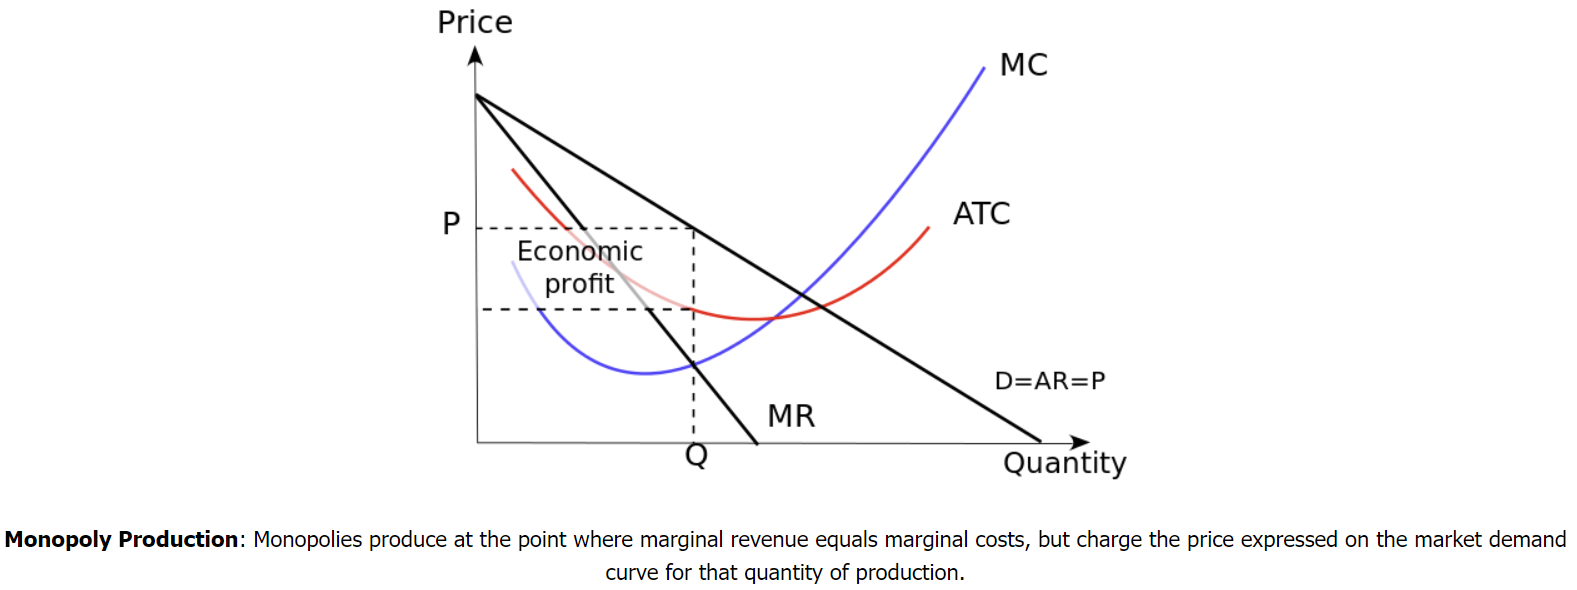
\includegraphics[width=16cm]{figures/Screenshot (98).png}
    \caption{The monopoly chooses the price on the demand curve which correponds to the quantity at the intersection of MR = MC (LibreTexts).}
\end{figure}

\subsection{Empirical Analysis}
Using the filtered Medicaid data, I examine associations between the reported number of manufacturers and spending per dosage unit and per claim. For each outcome, I estimate regressions with year fixed effects, with and without log prescription claims.

We can first look at some preliminary results. If we group the data by the number of total manufacturers and average the spending per dosage unit, we can see an interesting relationship: 

\begin{figure}[H]
    \centering
    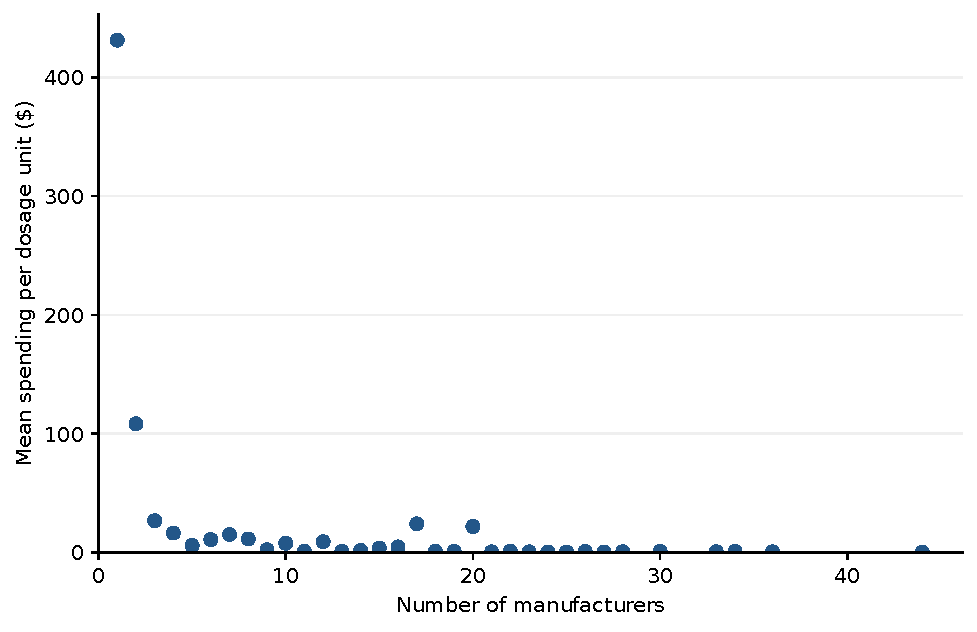
\includegraphics[width=13cm]{figures/medicaid_mean_spending.pdf}
    \caption{Scatterplot of the mean average spending per dosage unit of drugs (y-axis), grouped by number of manufacturers (x-axis).}
\end{figure}

The plot shows that mean spending per dosage unit is substantially lower for drugs with two or three manufacturers than for drugs with one manufacturer. Mean spending remains comparatively low at higher manufacturer counts, although it does not fall consistently as the count increases. These descriptive comparisons across drug groups provide suggestive evidence of a negative association between manufacturer counts and drug spending, but may reflect factors other than manufacturer counts.

\newpage

\subsubsection{Regression Analysis}

For our regression specification, the outcomes are average spending per dosage unit and average spending per claim. For each outcome, I estimate

\[
Y_{it}=\alpha+\beta M_i+\gamma\log C_{it}+\lambda_t+u_{it},
\]
where $i$ denotes a drug group defined by brand name and generic name, $t$ denotes year, $Y_{it}$ is the natural logarithm of the spending outcome, $M_i$ is the reported manufacturer count, and $C_{it}$ is the number of prescription claims. Drugs with larger markets based on the number of prescription claims may attract more manufacturers and have different spending patterns. I include log prescription claims to adjust for differences in utilization across drug groups.

I estimate each model by unweighted pooled ordinary least squares, with and without the log-claims term. Year fixed effects $\lambda_t$ account for changes common to all drug groups, with 2017 as the reference year. Standard errors are clustered by drug group. The reported manufacturer count does not vary over time within a drug group in these data, so drug-group fixed effects would therefore absorb the manufacturer-count covariate, preventing separate estimation of $\beta$. The manufacturer-count coefficient is estimated from differences across drug groups, conditional on the included controls.

% Generated by python -m analysis.run; do not edit.
\begin{table}[!htbp]
\centering
\caption{\MakeUppercase{Manufacturer counts and log spending per dosage unit}}
\label{table:table1}
\begin{singlespace}
\small
\begin{minipage}{0.95\linewidth}
\begin{tabular*}{\linewidth}{@{\extracolsep{\fill}}lcc@{}}
\toprule
 & \multicolumn{2}{c}{Log spending per unit} \\
\cmidrule(l){2-3}
 & (1) & (2) \\
\midrule
Number of manufacturers & $-0.186^{***}$ & $-0.130^{***}$ \\
 & (0.008) & (0.011) \\
\addlinespace[5pt]
Log prescription claims &  & $-0.173^{***}$ \\
 &  & (0.022) \\
\addlinespace[5pt]
Constant & $2.221^{***}$ & $3.655^{***}$ \\
 & (0.062) & (0.185) \\
\midrule
Year fixed effects & Yes & Yes \\
Drug fixed effects & No & No \\
Observations & 12,740 & 12,740 \\
Drug groups & 3,244 & 3,244 \\
$R^2$ & 0.110 & 0.127 \\
Adjusted $R^2$ & 0.110 & 0.127 \\
\bottomrule
\end{tabular*}
\par\vspace{5pt}
\begin{minipage}{\linewidth}
\footnotesize
\raggedright
\textit{Notes:} OLS with year indicators for 2017--2021 (2017 omitted). Drug groups are brand-name/generic-name pairs. Standard errors in parentheses are clustered by drug group, with a finite-sample correction. Tests use a $t$ distribution with the number of groups minus one degrees of freedom. Manufacturer counts are time-invariant in these data.
Per-unit spending is the reported weighted average per dosage unit.
All logarithms are natural.
$^{*}p<0.10$; $^{**}p<0.05$; $^{***}p<0.01$.
\end{minipage}
\end{minipage}
\end{singlespace}
\end{table}

\FloatBarrier

% Redundant total-spending table removed; associated prose awaits manual revision. 
\FloatBarrier

% Generated by python -m analysis.run; do not edit.
\begin{table}[!ht]
\centering
\caption{\MakeUppercase{Manufacturer counts and log spending per prescription claim}}
\label{table:table3}
\begin{singlespace}
\small
\begin{minipage}{0.95\linewidth}
\begin{tabular*}{\linewidth}{@{\extracolsep{\fill}}lcc@{}}
\toprule
 & \multicolumn{2}{c}{Log spending per claim} \\
\cmidrule(l){2-3}
 & (1) & (2) \\
\midrule
Number of manufacturers & $-0.170^{***}$ & $-0.091^{***}$ \\
 & (0.007) & (0.008) \\
\addlinespace[5pt]
Log prescription claims &  & $-0.245^{***}$ \\
 &  & (0.016) \\
\addlinespace[5pt]
Constant & $5.795^{***}$ & $7.829^{***}$ \\
 & (0.049) & (0.143) \\
\midrule
Year fixed effects & Yes & Yes \\
Drug fixed effects & No & No \\
Observations & 12,740 & 12,740 \\
Drug groups & 3,244 & 3,244 \\
$R^2$ & 0.147 & 0.203 \\
Adjusted $R^2$ & 0.147 & 0.202 \\
\bottomrule
\end{tabular*}
\par\vspace{5pt}
\begin{minipage}{\linewidth}
\footnotesize
\raggedright
\textit{Notes:} OLS with year indicators for 2017--2021 (2017 omitted). Drug groups are brand-name/generic-name pairs. Standard errors in parentheses are clustered by drug group, with a finite-sample correction. Tests use a $t$ distribution with the number of groups minus one degrees of freedom. Manufacturer counts are time-invariant in these data.
All logarithms are natural.
$^{*}p<0.10$; $^{**}p<0.05$; $^{***}p<0.01$.
\end{minipage}
\end{minipage}
\end{singlespace}
\end{table}

\FloatBarrier

The regressions in column (1) of each table have a negative sign on the manufacturer-count coefficient, which is what we expect based on economic theory. In particular, an increase in one manufacturer is associated with a 16.9\% decrease in the average spend per dosage unit and a 15.6\% decrease in the average spend per claim, controlling for year effects.

As seen in the regression tables, adding the natural logarithm of total claims reduces the magnitude of the manufacturer-count coefficients and increases $R^2$ for both outcomes.

In regression (2) for average spend per dosage unit (\autoref{table:table1}), adding log prescription claims increases $R^2$ from 0.110 to 0.127, and the adjusted $R^2$ is 0.127. Regression (2) indicates a negative association between the number of manufacturers and average spend per dosage unit. The coefficient on the number of manufacturers is smaller in magnitude after adding log prescription claims, but remains statistically significant at the 1\% level using standard errors clustered by drug group. The coefficient indicates that one additional manufacturer is associated with a 12.2\% decrease in average spend per dosage unit, holding the included controls constant. Additionally, the coefficient on log prescription claims is -0.173, indicating that a 1\% increase in total claims is associated with approximately a 0.173\% decrease in average spend per dosage unit, holding the other included covariates constant. 

Looking at regression (2) for average cost per claim (\autoref{table:table3}), we can see that adding log prescription claims increases $R^2$ from 0.147 to 0.203, and the adjusted $R^2$ is 0.202. One additional manufacturer is associated with an 8.7\% decrease in average spend per claim, holding the included controls constant. The manufacturer-count coefficient is statistically significant at the 1\% level. The coefficient on log prescription claims is -0.245, indicating that a 1\% increase in total claims is associated with approximately a 0.245\% decrease in average spend per claim, holding the other included covariates constant. This is a similar result to \autoref{table:table1}.

In summary, manufacturer counts are negatively associated with both measures of Medicaid drug spending, consistent with the economic theory and generic-entry literature discussed above. Manufacturers choose which drug markets to enter, and these decisions may depend on characteristics that also affect spending. The estimates therefore describe conditional associations across drug groups rather than causal effects of additional manufacturers. 

\section{Conclusion}
The Medicaid regressions show a negative association between manufacturer counts and average spending per dosage unit and per claim. Controlling for year fixed effects and log prescription claims, one additional manufacturer is associated with 12.2\% lower spending per dosage unit and 8.7\% lower spending per claim. These findings are consistent with the economic theory and generic-entry literature discussed above, but do not establish the causal effect of manufacturer entry.

The Medicaid findings point to competition as a potential means of improving drug affordability. If the observed relationship reflects competitive pressure, reducing obstacles to manufacturer entry could help contain spending on existing medicines. This possibility connects the results to the broader challenge of preserving incentives for pharmaceutical innovation while maintaining affordable access to treatment. For a publicly financed program, understanding this relationship is important for the cost of providing drug coverage. By constructing a panel from public Medicaid records, this paper contributes evidence on the relationship between market structure and Medicaid spending for drugs. Further research into why some drug markets attract more manufacturers than others could help establish when policies that encourage entry of manufacturers lead to lower spending. Understanding this could also help clarify how market characteristics shape entry decisions and inform research designs aimed at identifying the causal effect of entry on spending. Causal estimates would provide a stronger basis for evaluating policies that encourage competition.

